%%%%%%%%%%%%%%%%%%%%%%%%%%%%%%%%%%%%%%%%%
% Short Sectioned Assignment LaTeX Template Version 1.0 (5/5/12)
% This template has been downloaded from: http://www.LaTeXTemplates.com
% Original author:  Frits Wenneker (http://www.howtotex.com)
% License: CC BY-NC-SA 3.0 (http://creativecommons.org/licenses/by-nc-sa/3.0/)
%%%%%%%%%%%%%%%%%%%%%%%%%%%%%%%%%%%%%%%%%

%----------------------------------------------------------------------------------------
%	PACKAGES AND OTHER DOCUMENT CONFIGURATIONS
%----------------------------------------------------------------------------------------

\documentclass[paper=a4, fontsize=11pt]{scrartcl} % A4 paper and 11pt font size

% ---- Entrada y salida de texto -----

\usepackage[T1]{fontenc} % Use 8-bit encoding that has 256 glyphs
\usepackage[utf8]{inputenc}
%\usepackage{fourier} % Use the Adobe Utopia font for the document - comment this line to return to the LaTeX default

% ---- Idioma --------

\usepackage[spanish, es-tabla]{babel} % Selecciona el español para palabras introducidas automáticamente, p.ej. "septiembre" en la fecha y especifica que se use la palabra Tabla en vez de Cuadro

% ---- Otros paquetes ----
\usepackage{alltt}
\usepackage{hyperref}
\usepackage{url} % ,href} %para incluir URLs e hipervínculos dentro del texto (aunque hay que instalar href)
\usepackage{amsmath,amsfonts,amsthm} % Math packages
%\usepackage{graphics,graphicx, floatrow} %para incluir imágenes y notas en las imágenes
\usepackage{graphics,graphicx, float} %para incluir imágenes y colocarlas

\usepackage{cite}
\usepackage{listings}
\usepackage{xcolor}

% Para hacer tablas comlejas
%\usepackage{multirow}
%\usepackage{threeparttable}

%\usepackage{sectsty} % Allows customizing section commands
%\allsectionsfont{\centering \normalfont\scshape} % Make all sections centered, the default font and small caps

\usepackage{fancyhdr} % Custom headers and footers

\setcounter{secnumdepth}{0}
\pagestyle{fancyplain} % Makes all pages in the document conform to the custom headers and footers
\fancyhead{} % No page header - if you want one, create it in the same way as the footers below
\fancyfoot[L]{} % Empty left footer
\fancyfoot[C]{} % Empty center footer
\fancyfoot[R]{\thepage} % Page numbering for right footer
\renewcommand{\headrulewidth}{0pt} % Remove header underlines
\renewcommand{\footrulewidth}{0pt} % Remove footer underlines
\setlength{\headheight}{13.6pt} % Customize the height of the header

\numberwithin{equation}{section} % Number equations within sections (i.e. 1.1, 1.2, 2.1, 2.2 instead of 1, 2, 3, 4)
\numberwithin{figure}{section} % Number figures within sections (i.e. 1.1, 1.2, 2.1, 2.2 instead of 1, 2, 3, 4)
\numberwithin{table}{section} % Number tables within sections (i.e. 1.1, 1.2, 2.1, 2.2 instead of 1, 2, 3, 4)

\setlength\parindent{0pt} % Removes all indentation from paragraphs - comment this line for an assignment with lots of text

\newcommand{\horrule}[1]{\rule{\linewidth}{#1}} % Create horizontal rule command with 1 argument of height


%----------------------------------------------------------------------------------------
%	TÍTULO Y DATOS DEL ALUMNO
%----------------------------------------------------------------------------------------

\title{	
\normalfont \normalsize 
\textsc{\textbf{Ingeniería de Servidores (2016-2017)} \\ Grado en Ingeniería Informática \\ Universidad de Granada} \\ [25pt] % Your university, school and/or department name(s)
\horrule{0.5pt} \\[0.4cm] % Thin top horizontal rule
\huge Memoria Práctica 3 \\ % The assignment title
\horrule{2pt} \\[0.5cm] % Thick bottom horizontal rule
}

\author{José Álvaro Garrido López} % Nombre y apellidos

\date{\normalsize\today} % Incluye la fecha actual

%----------------------------------------------------------------------------------------
% DOCUMENTO
%----------------------------------------------------------------------------------------

\begin{document}
\maketitle % Muestra el Títuolo

\newpage %inserta un salto doe página

\tableofcontents % para generar el índice de contenidos

\listoffigures

\newpage

\newpage

\section{Cuestión 1.}

\subsection{a) ¿Qué archivo le permite ver qué programas se han instalado con el gestor de paquetes?}

En el caso de \textbf{CentOS}, como se menciona en \cite{yum}, existe un fichero llamado \textit{yum.log} donde se almacenan todas las acciones que se realizan sobre el comando \textit{yum}. En \ref{yumlog} se puede ver un fragmento del log.

\begin{figure}[H]
	\centering
	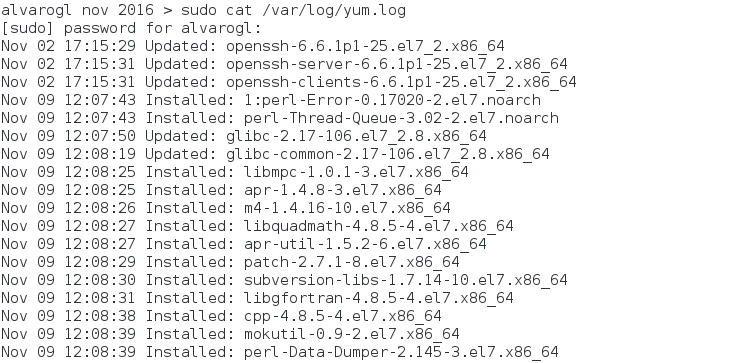
\includegraphics[scale=0.6]{cuestion1-yumlog.png}
	\caption{Fragmento del fichero \textit{/var/log/yum.log}} \label{yumlog}
\end{figure}

También, como se explica en el guión de prácticas, tenemos una alternativa con interfaz gráfica, \textit{\textit{gnome-system-log}}.
Ejecutamos \begin{verbatim}
gnome-system-log
\end{verbatim} desde terminal, y nos aparece la ventana que se observa en \ref{gnome-system-log}.

\begin{figure}[H]
	\centering
	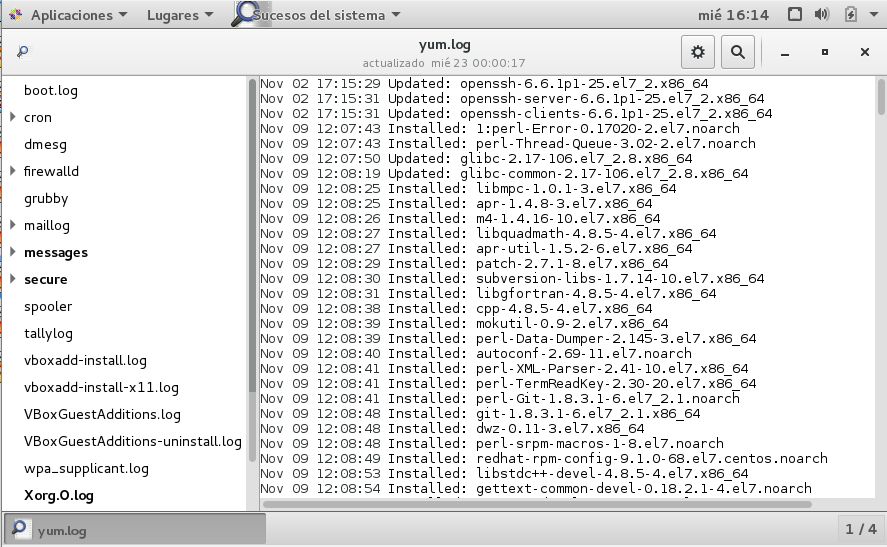
\includegraphics[scale=0.6]{cuestion1-gnomesyslog.png}
	\caption{Captura de la interfaz gráfica de \textbf{\textit{gnome-system-log}}} \label{gnome-system-log}
\end{figure}

Si desplegamos en la interfaz el fichero \textit{yum.log}, como se muestra en \ref{gnome-system-log2}, podemos comprobar que el programa nos ordena por fecha las entradas del fichero, lo cual puede ser de gran utilidad.

\begin{figure}[H]
	\centering
	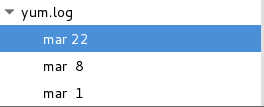
\includegraphics[scale=0.6]{cuestion1-gnomesyslog2.png}
	\caption{Captura de selección por fecha en \textbf{\textit{gnome-system-log}}} \label{gnome-system-log2}
\end{figure}

En el caso de \textbf{Ubuntu}, en \cite{debian}, se nos explica que existen varios ficheros históricos que almacenan la actividad de \textit{apt}, como lo son \textit{/var/log/dpkg.log}, \textit{/var/log/apt/term.log} y \textit{/var/log/aptitude}. El más conciso de ellos es \textit{/var/log/apt/term.log}, aunque también existe otro archivo que se menciona en \cite{ubuntubook}, \textit{/var/log/apt/history.log}, cuyo contenido podemos ver en \ref{historylog} que almacena los comandos ejecutados sobre \textit{apt}.

\begin{figure}[H]
	\centering
	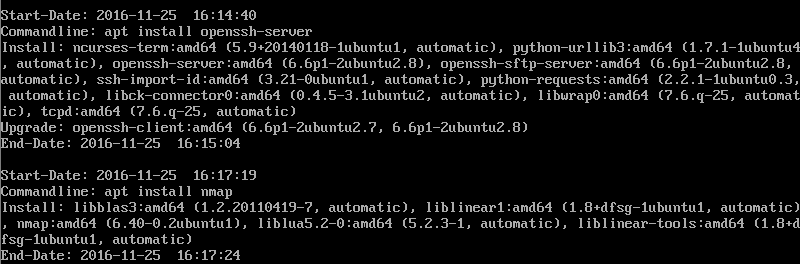
\includegraphics[scale=0.6]{cuestion1-historylog.png}
	\caption{Captura del archivo \textit{/var/log/apt/history.log}} \label{historylog}
\end{figure}

\subsection{b) ¿Qué significan las terminaciones 1.gz o 2.gz de los archivos en ese directorio?}

Podemos descomprimir estos archivos ejecutando el siguiente comando:
\begin{verbatim}
gunzip /var/log/archivo.gz
\end{verbatim}

En \cite{gunzip} se explica el uso del comando \textit{gunzip}.

En \cite{compression} se habla del problema que acarrea el tamaño de los logs del sistema, y que una opción es comprimir estos archivos en formato \textit{.gz}.

Podemos ver un fragmento del archivo \textit{/var/log/dmesg.1.gz} descomprimido en \ref{dmesg1}.

\begin{figure}[H]
	\centering
	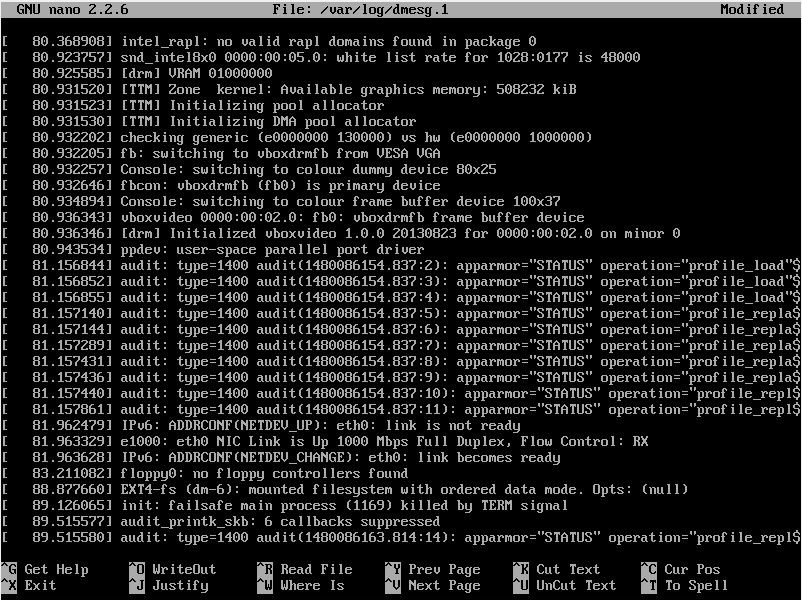
\includegraphics[scale=0.45]{cuestion1-gznano.png}
	\caption{Captura del archivo \textit{/var/log/dmes.1.gz} descomprimido} \label{dmesg1}
\end{figure}

\section{Cuestión 2. ¿Qué archivo ha de modificar para programar una tarea? Escriba la línea necesaria para ejecutar una vez al día una copia del directorio ~/codigo a ~/seguridad/\$fecha donde \$fecha es la fecha actual (puede usar el comando date)}

Como se explica en \cite{cron} y \cite{cron2}, través del comando: \begin{verbatim}
sudo crontab -e <usuario>
\end{verbatim}

podemos editar el fichero para programar tareas.
Por defecto se nos asigna un archivo \textit{crontab} en \textit{/tmp}, pero también tenemos acceso a \textit{/etc/cron.hourly}, \textit{/etc/cron.daily}, \textit{/etc/cron.weekly} y \textit{/etc/cron.monthly}.

Debemos añadir una línea con la siguiente sintaxis:

\begin{verbatim}
<minuto> <hora> <día del mes> <mes> <día de la semana> <comando>
\end{verbatim}

En concreto, para lo que se nos pide, tendríamos que añadir las siguientes línea:

\begin{verbatim}
DATE=date + %F
59 23 * * *  cp ~/codigo ~/seguridad/$($DATE)
\end{verbatim}

En concreto, utilizamos la opción +\%F de \textit{date} para que el nombre de la carpeta sea del tipo \textit{aaaa-mm-dd} y no contenga espacios, consultada la referencia \cite{date} para comprender la sintaxis del comando.

Para probar el funcionamiento de lo que se pregunta en la cuestión, he añadido la tarea \textit{cron} para que se ejecute cada minuto como se muestra en \ref{crontab}.
l
\begin{figure}[H]
	\centering
	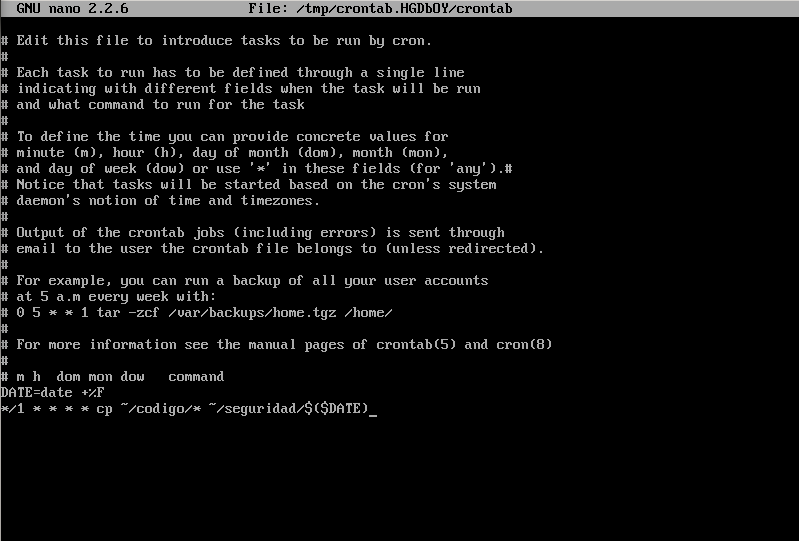
\includegraphics[scale=0.6]{cuestion2-crontab.png}
	\caption{Captura del fichero \textit{crontab}} \label{crontab}
\end{figure}  

En \ref{resultado-cron}, se comprueba el funcionamiento de lo descrito en la cuestión.

\begin{figure}[H]
	\centering
	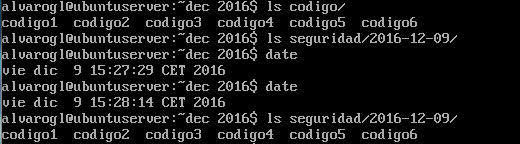
\includegraphics[scale=0.6]{cuestion2-resultado.png}
	\caption{Funcionamiento del fichero \textit{crontab} editado} \label{resultado-cron}
\end{figure}

\section{Cuestión 3. Pruebe a ejecutar el comando, conectar un dispositivo USB y vuelva a ejecutar el comando. Copie y pegue la salida del comando. (Considere usar dmesg | tail). Comente qué observa en la información mostrada}

Según \cite{dmesg}, para que se muestre la fecha y la hora de los mensajes de diagnóstico, debemos utilizar la opción -F del comando.

En \ref{cuestion3-usb} se muestran los mensajes de diagnóstico antes de introducir el USB y en \ref{cuestion3-usb2} después de hacerlo.

\begin{figure}[H]
	\centering
	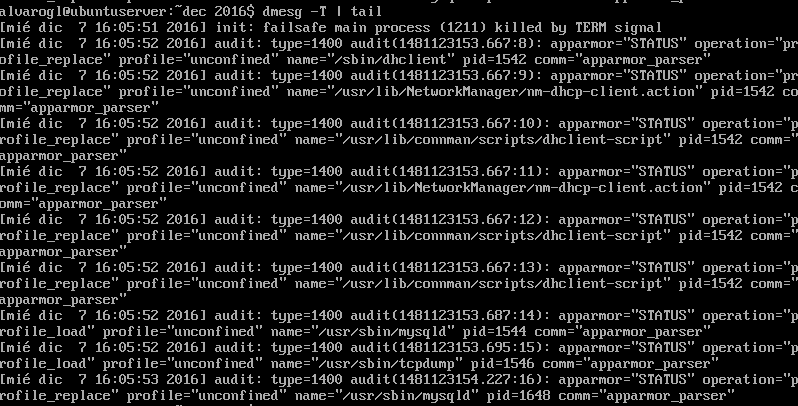
\includegraphics[scale=0.6]{cuestion3-usb.png}
	\caption{Ejecución del comando \textit{dmesg} antes de introducir el \textit{USB}} \label{cuestion3-usb}
\end{figure}

\begin{figure}[H]
	\centering
	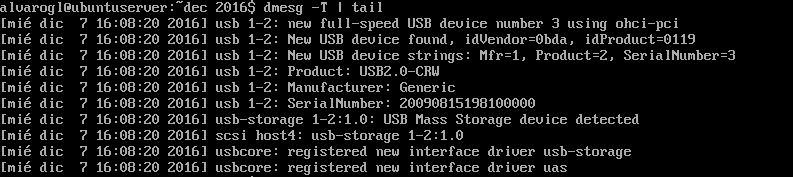
\includegraphics[scale=0.6]{cuestion3-usb2.png}
	\caption{Ejecución del comando \textit{dmesg} después de introducir el \textit{USB}} \label{cuestion3-usb2}
\end{figure}

Como podemos apreciar en \ref{cuestion3-usb2}, los mensajes de diagnóstico son sensibles a la conexión de un nuevo dispositivo por \textit{USB}.  Se indican entre otros parámetros, el fabricante, el número de serie y el nombre del dispositivo.

Si esperamos unos segundos nos aparece más información sobre el montaje del dispositivo. En \ref{cuestion3-usb3} se especifican los bloques lógicos y el espacio en GB del dispositivo, la protección de escritura desactivada y otras cuestiones.

\begin{figure}[H]
	\centering
	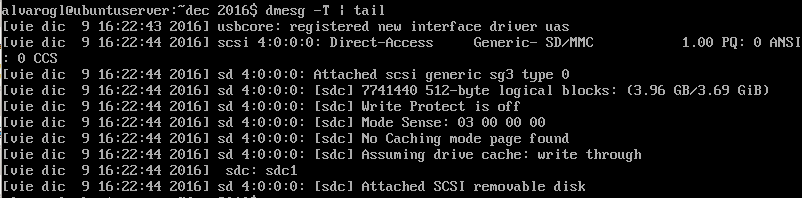
\includegraphics[scale=0.6]{cuestion3-usb3.png}
	\caption{Mensajes de diagnóstico segundos después} \label{cuestion3-usb3}
\end{figure}

\newpage

\section{Cuestión 4. Ejecute el monitor de $"$System Performance$"$ y muestre el resultado. Incluya capturas de pantalla comentando la información que aparece}

Ejecutamos el \textbf{System Performance} como se muestra en \ref{cuestion4-inicio}

\begin{figure}[H]
	\centering
	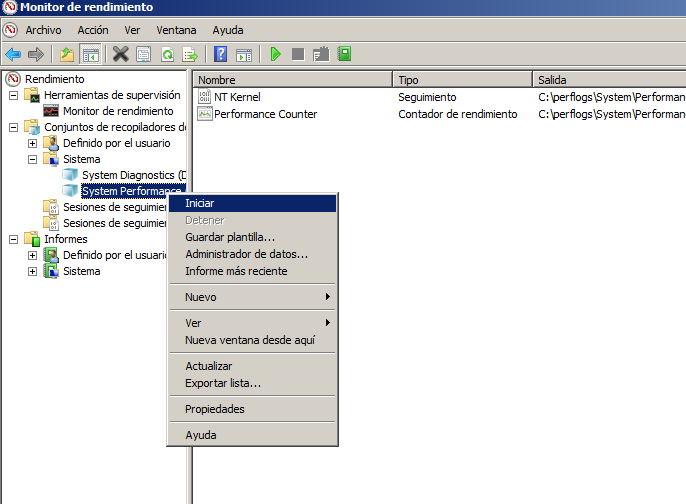
\includegraphics[scale=0.6]{cuestion4-inicio.png}
	\caption{Inicio de \textbf{System Performance}} \label{cuestion4-inicio}
\end{figure}

A continuación vemos el informe y algunos de los aspectos más llamativos.
En \ref{informe-rendimiento} aparece la primera vista del informe.

\begin{figure}[H]
	\centering
	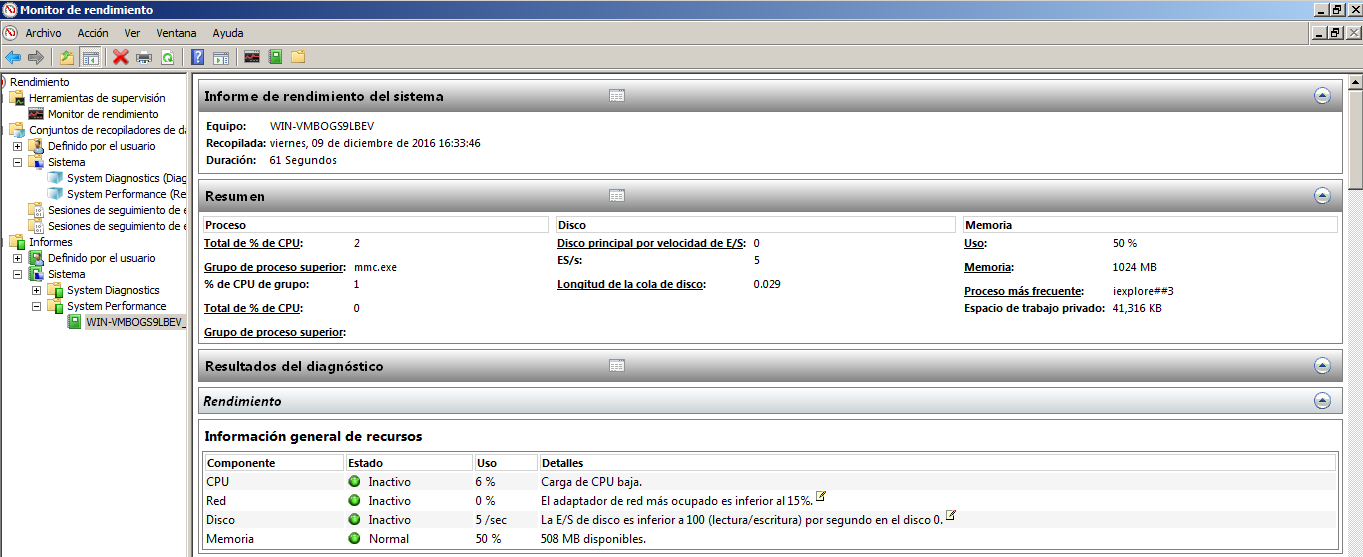
\includegraphics[scale=0.35]{cuestion4-1.png}
	\caption{Informe de rendimiento del sistema en \textbf{System Performance}} \label{informe-rendimiento}
\end{figure}

En \ref{cuestion4-cpuproceso} se pueden ver cuáles son los procesos y en qué porcentaje usan a la CPU.

\begin{figure}[H]
	\centering
	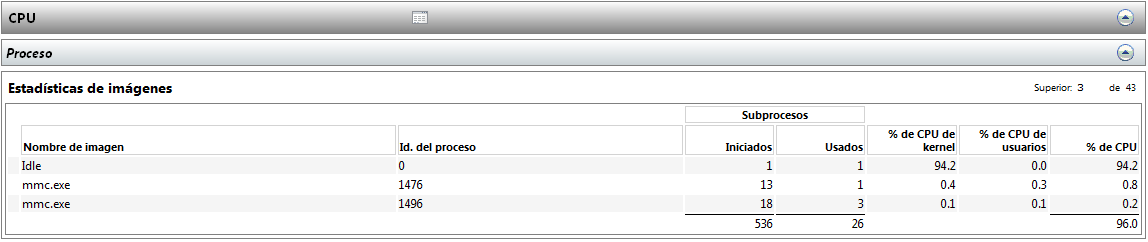
\includegraphics[scale=0.35]{cuestion4-2.png}
	\caption{Apartado \textit{CPU} del informe} \label{cuestion4-cpuproceso}
\end{figure}

En \ref{cuestion4-procesador} se nos proporciona información referente al procesador. Aparecen el número medio de interrupciones, porcentaje de inactividad, porcentaje de ejecución de procesos en modo usuario y en modo privilegiado, etc.

\begin{figure}[H]
	\centering
	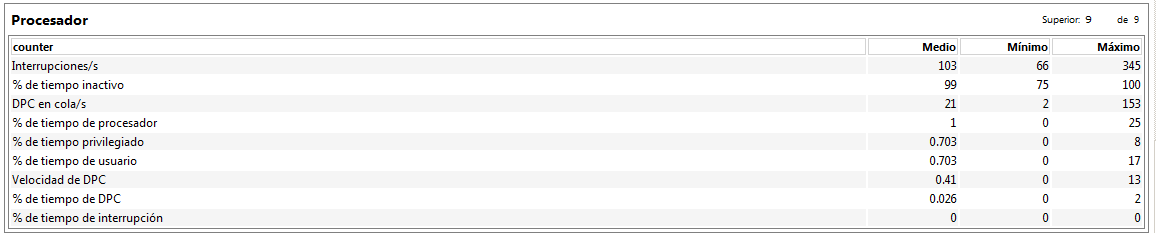
\includegraphics[scale=0.35]{cuestion4-3.png}
	\caption{Información sobre el procesador en el informe} \label{cuestion4-procesador}
\end{figure}

En \ref{cuestion4-servicios} se nos listan los servicios del sistema, el \textit{processId}, y el porcentaje de CPU.

\begin{figure}[H]
	\centering
	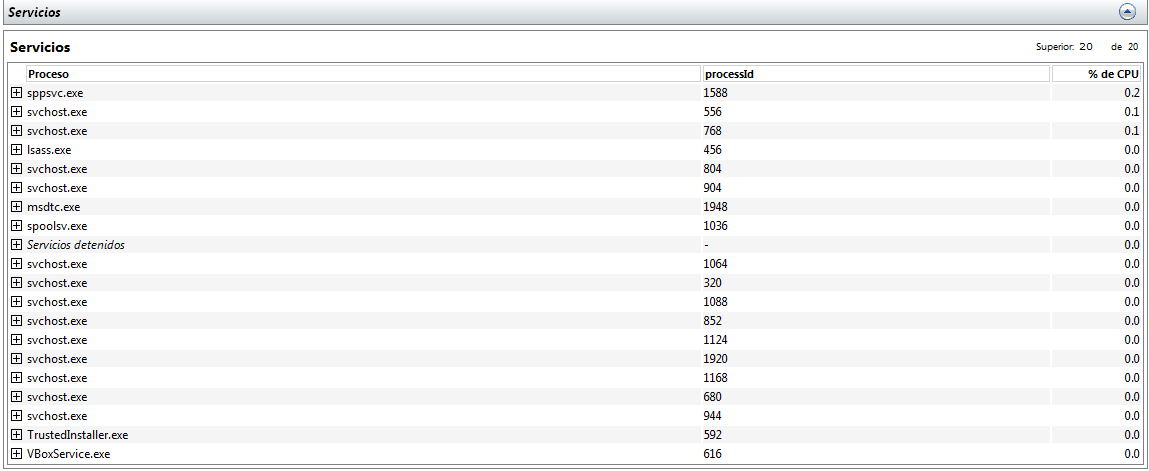
\includegraphics[scale=0.35]{cuestion4-4.png}
	\caption{Servicios del sistema} \label{cuestion4-servicios}
\end{figure}

En \ref{cuestion4-memoria} aparecen información de los procesos en cuanto a la memoria que están utilizando.

\begin{figure}[H]
	\centering
	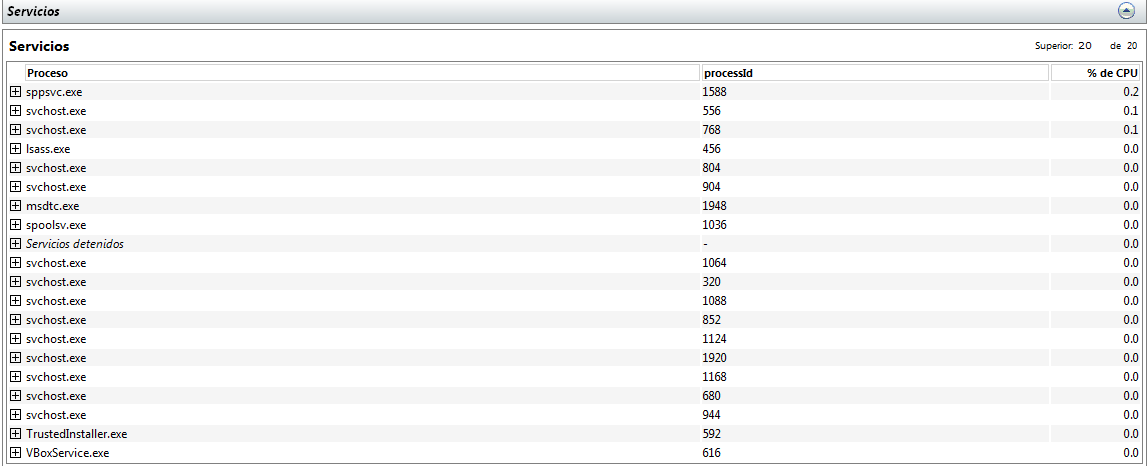
\includegraphics[scale=0.35]{cuestion4-5.png}
	\caption{Información sobre el uso de memoria en el sistema} \label{cuestion4-memoria}
\end{figure}

En \ref{cuestion4-estadisticas} se detallan estadísticas del informe, así como información del equipo, velocidad del procesador, cantidad de memoria, arquitectura del procesador y otros parámetros.

\begin{figure}[H]
	\centering
	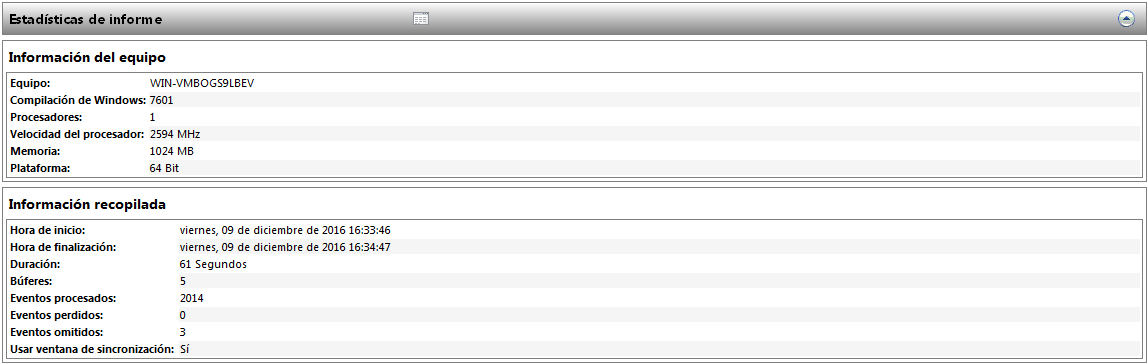
\includegraphics[scale=0.35]{cuestion4-7.png}
	\caption{Estadísticas del informe} \label{cuestion4-estadisticas}
\end{figure}

\section{Cuestión 5. Cree un recopilador de datos definido por el usuario (modo avanzado) que incluya tanto el contador de rendimiento como los datos de seguimiento: Todos los referentes al procesador, al proceso y al servicio web. Intervalo de muestra 15 segundos. Almacene el resultado en el directorio Escritorio/logs. Incluya las capturas de pantalla de cada paso}

Siguiendo las indicaciones del enunciado de la cuestión, creamos un nuevo \textit{recopilador de datos} como se muestra en \ref{cuestion5-nuevoreco}.

\begin{figure}[H]
	\centering
	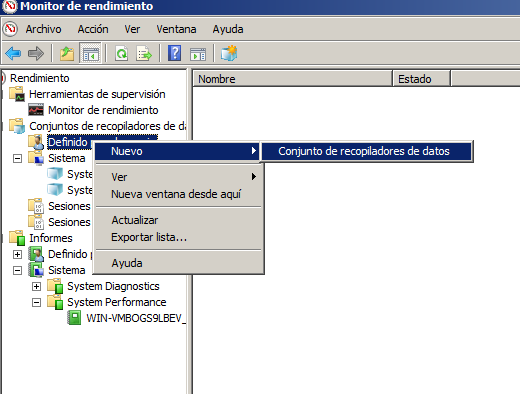
\includegraphics[scale=0.6]{cuestion5-nuevoreco.png}
	\caption{Creación de un nuevo conjunto de \textit{recopiladores de datos}} \label{cuestion5-nuevoreco}
\end{figure}

Posteriormente, como se muestra en \ref{cuestion5-crear-reg}, seleccionamos la opción \textbf{Crear registro de datos}, marcamos el contador de rendimiento y los datos de seguimiento. La información de configuración del sistema es opcional.

\begin{figure}[H]
	\centering
	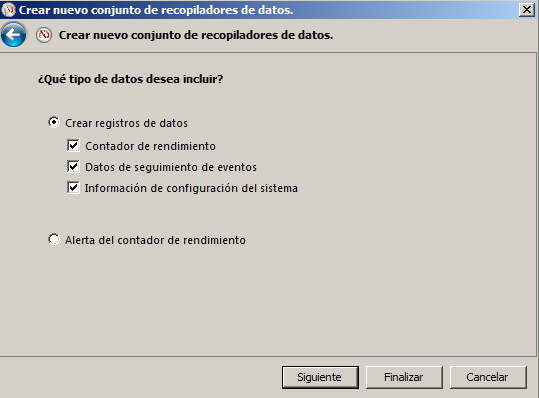
\includegraphics[scale=0.6]{cuestion5-crear-reg.png}
	\caption{\textit{Wizard} de creación del recopilador} \label{cuestion5-crear-reg}
\end{figure}

Para agregar contadores, en el \textit{Wizard}, como se ve en \ref{cuestion5-agregar-contador}, buscamos el contador que deseemos y agregamos todas las instancias del objeto seleccionado. Al final deben quedar agregados los contadores referentes a procesador, proceso y servicio web.

\begin{figure}[H]
	\centering
	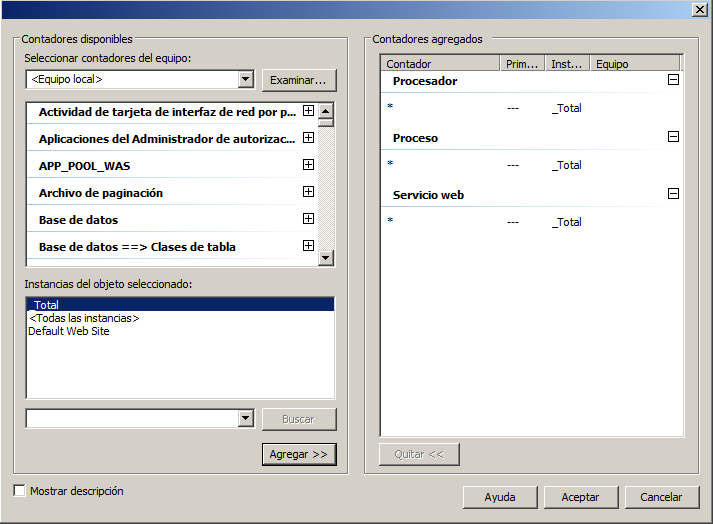
\includegraphics[scale=0.6]{cuestion5-agregar-contador.png}
	\caption{Adición de contadores referentes al procesador, proceso y servicio web} \label{cuestion5-agregar-contador}
\end{figure}

Para determinar el intervalo de muestra, en el paso referente a \ref{cuestion5-muestra}, indicamos el intervalo de 15 segundos.

\begin{figure}[H]
	\centering
	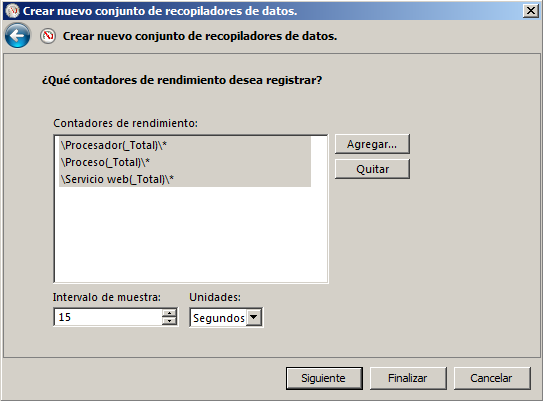
\includegraphics[scale=0.6]{cuestion5-muestra.png}
	\caption{Definición del intervalo de muestra para el recopilador} \label{cuestion5-muestra}
\end{figure}

Para terminar, almacenamos los datos en el \textit{/Desktop/logs}. Ver \ref{cuestion5-escritorio}.

\begin{figure}[H]
	\centering
	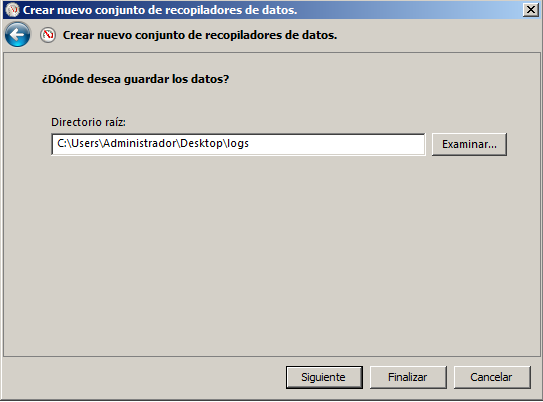
\includegraphics[scale=0.6]{cuestion5-escritorio.png}
	\caption{Almacenamiento de los datos en la carpeta \textit{logs} del escritorio} \label{cuestion5-escritorio}
\end{figure}

Como se observa en los resultados \ref{cuestion5-resultado}, el informe ha recaudado un montón de datos de compleja interpretación.
Si pinchamos en una zona del gráfico obtenido, nos aparecen debajo los colores identificadores de los datos que se encuentren en esa franja del gráfico. Por ejemplo, en \ref{cuestion5-resultado}, hay un pequeño pico en las operaciones de ES de dato/s.

\begin{figure}[H]
	\centering
	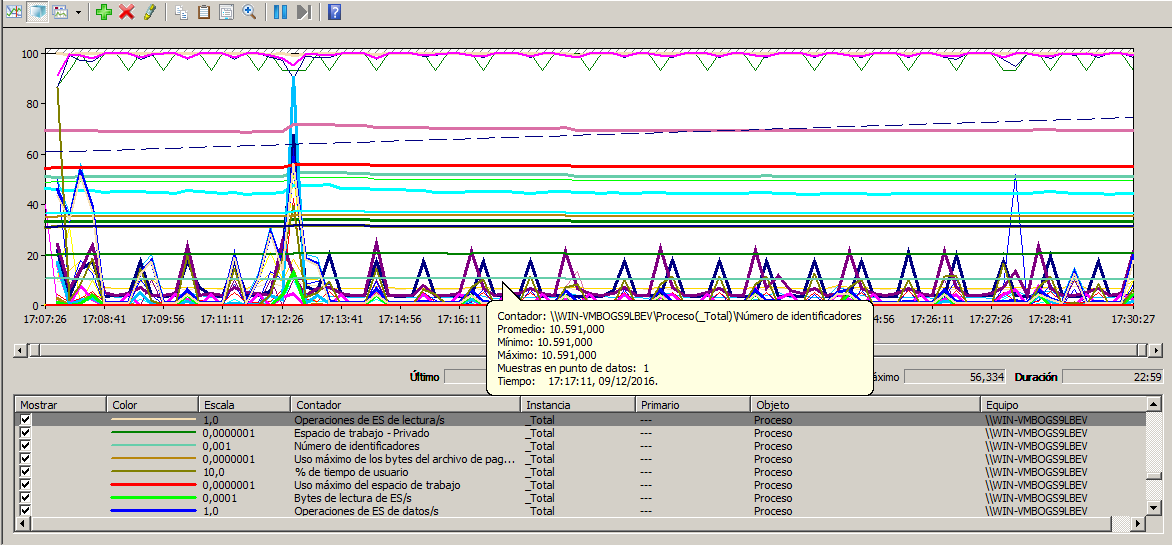
\includegraphics[scale=0.35]{cuestion5-resultado.png}
	\caption{Resultado del recopilador de datos} \label{cuestion5-resultado}
\end{figure}

Si pinchamos en algún identificador, como en \ref{cuestion5-pinchar} con las interrupciones, se nos muestra el último dato, el promedio, el mínimo, y el máximo.

\begin{figure}[H]
	\centering
	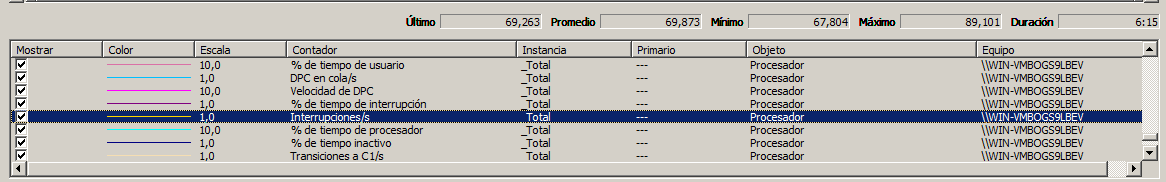
\includegraphics[scale=0.35]{cuestion5-pinchar.png}
	\caption{Identificadores del gráfico} \label{cuestion5-pinchar}
\end{figure}

En \ref{cuestion5-porcentaje-privilegiado}, podemos comprobar el porcentaje del tiempo que se ha ejecutado el procesador en modo privilegiado. En este caso ha sido casi del 100\%, el último dato registrado ha sido de 99,479\% y el promedio de 99,571\%.

\begin{figure}[H]
	\centering
	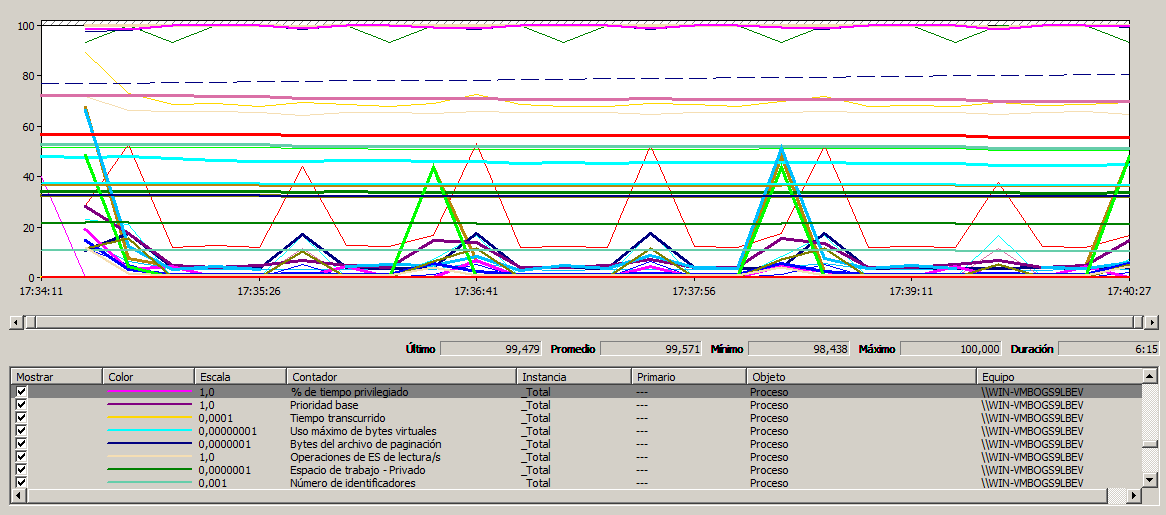
\includegraphics[scale=0.35]{cuestion5-porcentaje-privilegiado.png}
	\caption{Porcentaje de tiempo en modo privilegiado} \label{cuestion5-porcentaje-privilegiado}
\end{figure}

\section{Cuestión 6. Visite la web del proyecto y acceda a la demo que proporcionan (http://demo.munin-monitoring.org/) donde se muestra cómo monitorizan un servidor. Monitorice varios parámetros y haga capturas de pantalla de lo que está mostrando comentando qué observa.}

La demo de \textbf{Munin} se encuentra en \cite{munin}.
En \ref{cuestion6-overview} se muestra la vista general de \textbf{Munin}, donde se pueden ver algunas de las funcionalidades de las que dispone esta herramienta.
Podemos clasificar las estadísticas recogidas por día, semana, mes o año. En mi caso he utilizado los datos recopilados por año.

\begin{figure}[H]
	\centering
	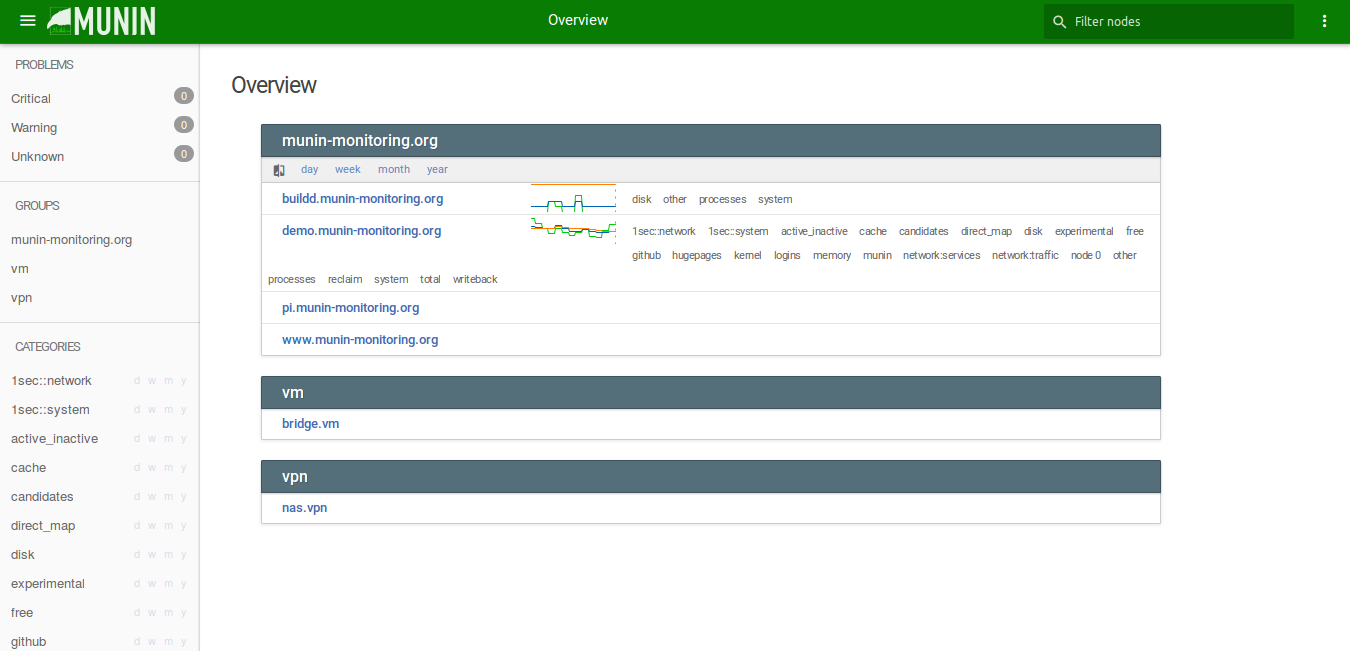
\includegraphics[scale=0.35]{cuestion6-overview.png}
	\caption{Vista general de \textbf{Munin}} \label{cuestion6-overview}
\end{figure}

Entre las estadísticas que podemos consultar, como se muestra en \ref{cuestion6-comparaciones}, se encuentran las referentes a la interfaz de red, al uso del disco, a la memoria, a los procesos, o al sistema.

\begin{figure}[H]
	\centering
	
\includegraphics[scale=0.45]{cuestion6-comparaciones.png}
	\caption{Gráficos de \textbf{Munin}, resultados por año} \label{cuestion6-comparaciones}
\end{figure}

Como se muestra en \ref{cuestion6-hebras}, en \textbf{Munin} se han utilizado como máximo 97 hebras en el último año, como promedio 70.

\begin{figure}[H]
	\centering
	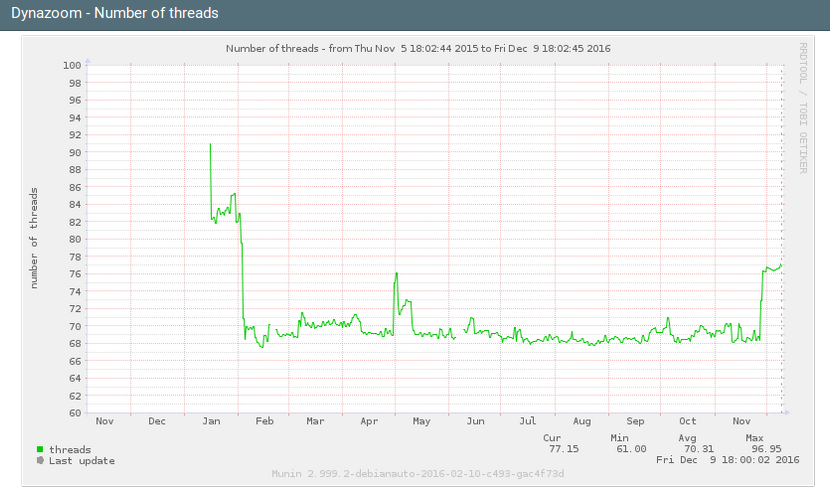
\includegraphics[scale=0.6]{cuestion6-hebras.png}
	\caption{Gráfico sobre el número de hebras utilizadas} \label{cuestion6-hebras}
\end{figure}

En \ref{cuestion6-interrupciones} se muestran las interrupciones dadas en el último año, así como los cambios de contexto que se han producido.

\begin{figure}[H]
	\centering
	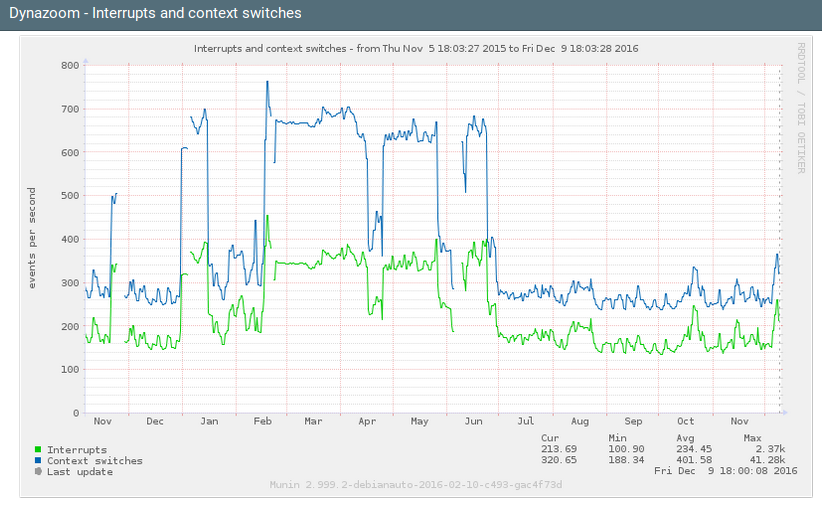
\includegraphics[scale=0.6]{cuestion6-interrupciones.png}
	\caption{Gráfico sobre interrupciones del sistema} \label{cuestion6-interrupciones}
\end{figure}

En \ref{cuestion6-memory} se muestra un gráfico detallado del uso de la memoria en el servidor. Entre otros datos se detallan el número de paginaciones, el \textit{swap}, memoria no utilizada, memoria \textit{mapeada}, activa e inactiva.

\begin{figure}[H]
	\centering
	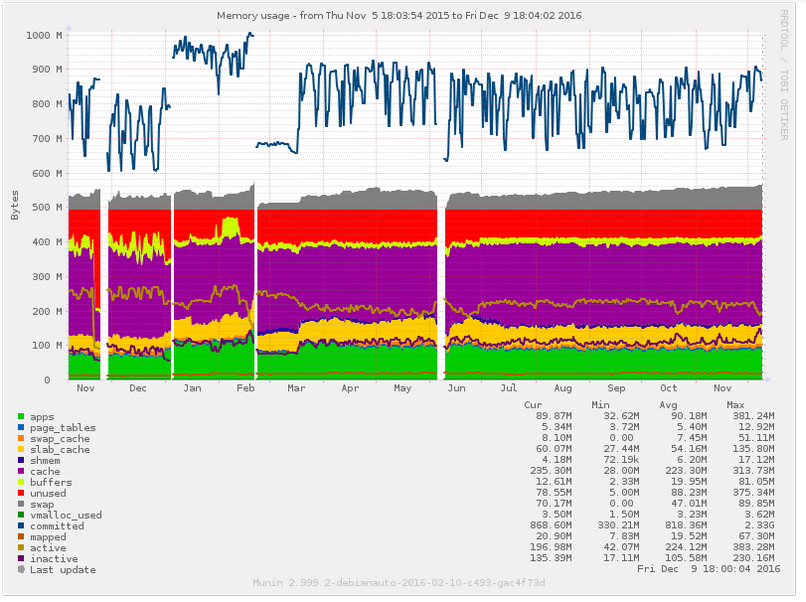
\includegraphics[scale=0.6]{cuestion6-memory.png}
	\caption{Gráfico sobre memoria utilizada} \label{cuestion6-memory}
\end{figure}

\section{Cuestión 7. Escriba un breve resumen sobre alguno de los artículos donde se muestra el uso de strace o busque otro y coméntelo}

He escogido el artículo que se encuentra en \cite{sysadmintips}.
En este, se habla de que son muchas las ocasiones en las que un administrador de sistema se ve en una situación en la que no sabe cómo ha ocurrido un determinado error, o un evento inesperado en el sistema, y no existe ningún fichero \textit{log} donde se expliquen dichos errores.
Para estos casos, la utilización de la herramienta \textbf{strace} es realmente potente para monitorizar llamadas al sistema y señales. Debe ser ejecutado con permisos de \textit{root} para aprovechar toda su funcionalidad.

En el artículo se nos describen casos concretos en los que \textbf{strace} tiene gran utilidad.
Por ejemplo, cuando no conocemos el fichero de \textit{logs} de una aplicación, sencillamente podemos seguir su traza y filtrar la misma con una concatenación de \textit{grep log}. De esta forma será muy fácil saber cuáles son los ficheros de \textit{log} de ese programa.

También podemos encontrar errores en la ejecución de un programa filtrando la traza del mismo con \textit{grep -1}, ya que esta es la forma que \textbf{strace} tiene de decirnos que en la ejecución de esa línea ha ocurrido un error.

\section{Cuestión 8. Escriba un script en Python o PHP y analice su comportamiento usando el profiler presentado}

El script que he utilizado se presenta a continuación (y será añadido al archivo comprimido de la entrega como \textit{prof.py}):

\begin{lstlisting}
#!/usr/bin/env python3
import profile

def fib(n):
	if n == 0:
		return 0

	elif n == 1:
		return 1

	else:
		return fib(n-1)+fib(n-2)

def loop():
	n = 0
	while n < 10000000:
		n = n+1

def main():
	print ("IN LOOP")
	loop()
	print("FIB(30)")
	fib(30)

profile.run('main()')
\end{lstlisting}

El código al que vamos a pasar el \textit{profiler} se resume en dos funciones en \textbf{Python}, una de ellas calcula el término \textit{n} de la sucesión de \textbf{Fibonacci}, y la otra es un bucle desde 0 hasta 10 millones dentro del cual se incrementa una variable.

Para analizar el comportamiento del mismo con el \textit{profiler} de \textbf{Python}, he recurrido a la biblioteca \textit{profile}, que se explica en \cite{python}.

Como podemos ver en \ref{cuestion8-profile1}, el bucle tarda 2.096 segundos en ejecutarse mientras que la función de \textbf{Fibonacci} tarda 13.593 segundos.

\begin{figure}[H]
	\centering
	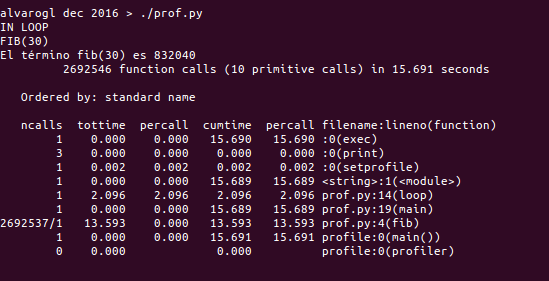
\includegraphics[scale=0.6]{cuestion8-profile1.png}
	\caption{Resultado del \textit{profile} de la primera versión} \label{cuestion8-profile1}
\end{figure}

Habría posibilidad de mejorar este código, ya que la función que más tiempo de ejecución consume es la de \textbf{Fibonacci}, pero existen otros algoritmos más eficientes para hacer este cálculo.

El script que he utilizado para mejorar el código se presenta a continuación (y será añadido al archivo comprimido de la entrega como \textit{prof\_mejora.py}):

\begin{lstlisting}
#!/usr/bin/env python3
import profile

def fib(n):
	a, b = 0, 1
	for _ in range(n):
		a, b = b, a+b
	return a

def loop():
	n = 0
	while n < 10000000:
		n = n+1

def main():
	print ("IN LOOP")
	loop()
	print("FIB(30)")
	fib(30)

profile.run('main()')
\end{lstlisting}

En este caso he utilizado una versión iterativa del algoritmo para calcular un término \textit{n} de \textbf{Fibonacci}, y el resultado, como se muestra en \ref{cuestion8-profile2}, es notablemente mejor, pues el tiempo de ejecución de \textbf{Fibonacci} es inferior a 1 milisegundo (el \textit{profiler} indica que el tiempo es de 0.000 segundos).

\begin{figure}[H]
	\centering
	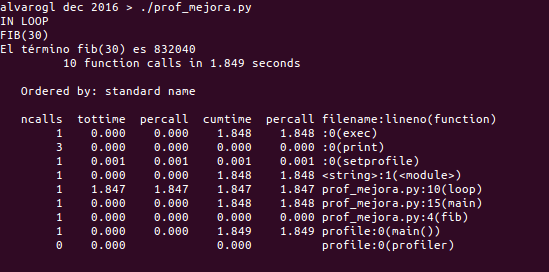
\includegraphics[scale=0.6]{cuestion8-profile2.png}
	\caption{Resultado del \textit{profile} de la segunda versión} \label{cuestion8-profile2}
\end{figure}

\section{Cuestión 9. Acceda a la consola mysql (o a través de phpMyAdmin) y muestre el resultado de mostrar el $"$profile$"$ de una consulta (la creación de la BD y la consulta la puede hacer libremente)}

En mi caso, he buscado una base de datos de ejemplo de la página oficial de \textbf{MySQL} que se puede encontrar en \cite{mysql-download}. En concreto, he escogido la de \textit{world}.

Se han consultado las referencias de \cite{mysql-profile} y \cite{mysql-profiles} para la realización del ejercicio.

En primer lugar, es necesario acceder a la base de datos, para ello, como se explica en \cite{mysql-guide}, ejecutamos:

\begin{verbatim}
mysql -uroot -p
\end{verbatim}

Para activar el \textit{profiling} se utiliza el \textit{mysql-command}:

\begin{verbatim}
set profiling = 1;
\end{verbatim}

Creamos la base de datos, la utilizamos e importamos \textit{world.sql}, que fue descargado de \cite{mysql-download} (dicho archivo será adjuntado al comprimido de la entrega). Lo hacemos de esta manera, como se ve en \ref{cuestion9-setprof-crear}:

\begin{verbatim}
create database world;
use world;
source world.sql
\end{verbatim}

\begin{figure}[H]
	\centering
	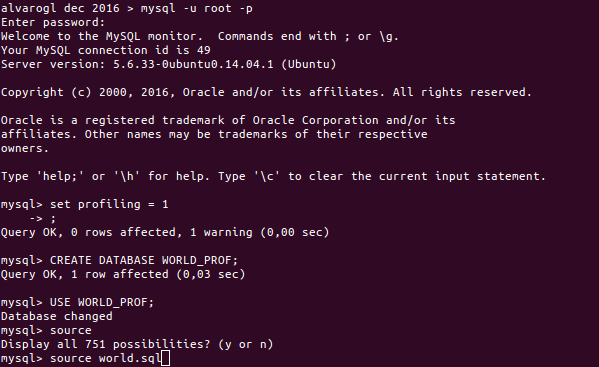
\includegraphics[scale=0.6]{cuestion9-setprof_crear.png}
	\caption{Creación y configuración del \textit{profiler}} \label{cuestion9-setprof-crear}
\end{figure}

Para comprobar los resultados del \textit{profile}, simplemente ejecutamos \textbf{SHOW PROFILES} para ver datos generales de la ejecución, como se aprecia en \ref{cuestion9-showprofiles}, y \textbf{SHOW PROFILE} (ver \ref{cuestion9-showprofile}) para incidir sobre una \textit{Query} en concreto.

\begin{figure}[H]
	\centering
	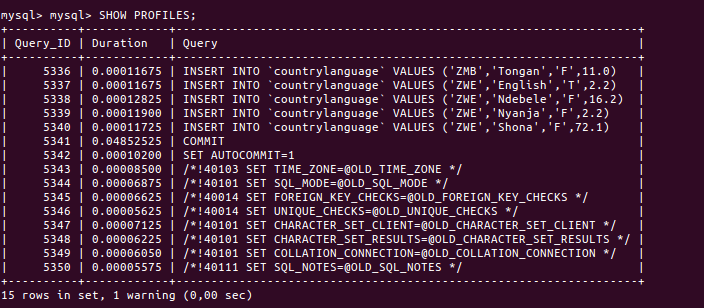
\includegraphics[scale=0.6]{cuestion9-showprofiles.png}
	\caption{Ejecución de \textbf{SHOW PROFILES}} \label{cuestion9-showprofiles}
\end{figure}

\begin{figure}[H]
	\centering
	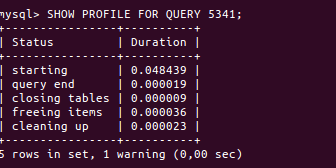
\includegraphics[scale=0.6]{cuestion9-showprofilecommit.png}
	\caption{Ejecución de \textbf{SHOW PROFILE}} \label{cuestion9-showprofile}
\end{figure}

He ejecutado dos ejemplos más para hacer un \textit{profiling} de la creación de una base de datos, en \ref{cuestion9-creacionbdprofiles} y otro de una consulta, en \ref{cuestion9-consulta}.

\begin{figure}[H]
	\centering
	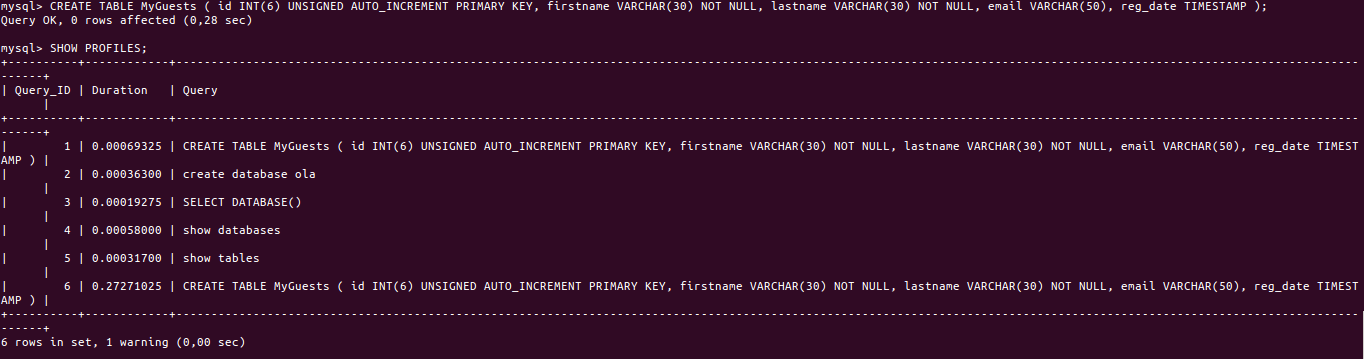
\includegraphics[scale=0.35]{cuestion9-creaciondbprofiles.png}
	\caption{\textit{Profile} de la creación de una base de datos} \label{cuestion9-creacionbdprofiles}
\end{figure}

\begin{figure}[H]
	\centering
	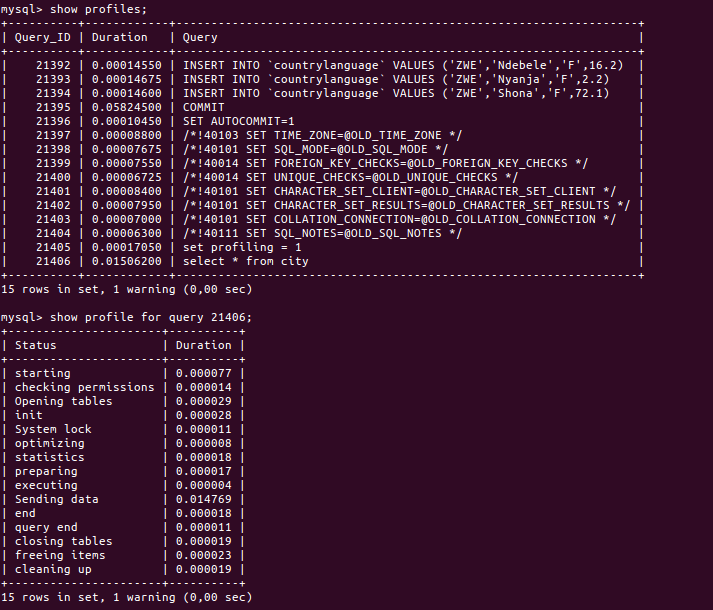
\includegraphics[scale=0.6]{cuestion9-consulta.png}
	\caption{\textit{Profile} de una consulta} \label{cuestion9-consulta}
\end{figure}

\newpage
\bibliographystyle{plain}
\bibliography{biblio}

\end{document}